\documentclass[border=5mm]{standalone}
\usepackage{luamplib}
\usepackage{graphicx}
\mplibtextextlabel{enable}
\begin{document}

    \begin{mplibcode}

        input segments.mp ;
        input waypoints.mp ;

        beginfig(0);
        picture A,B;
        A = TEX("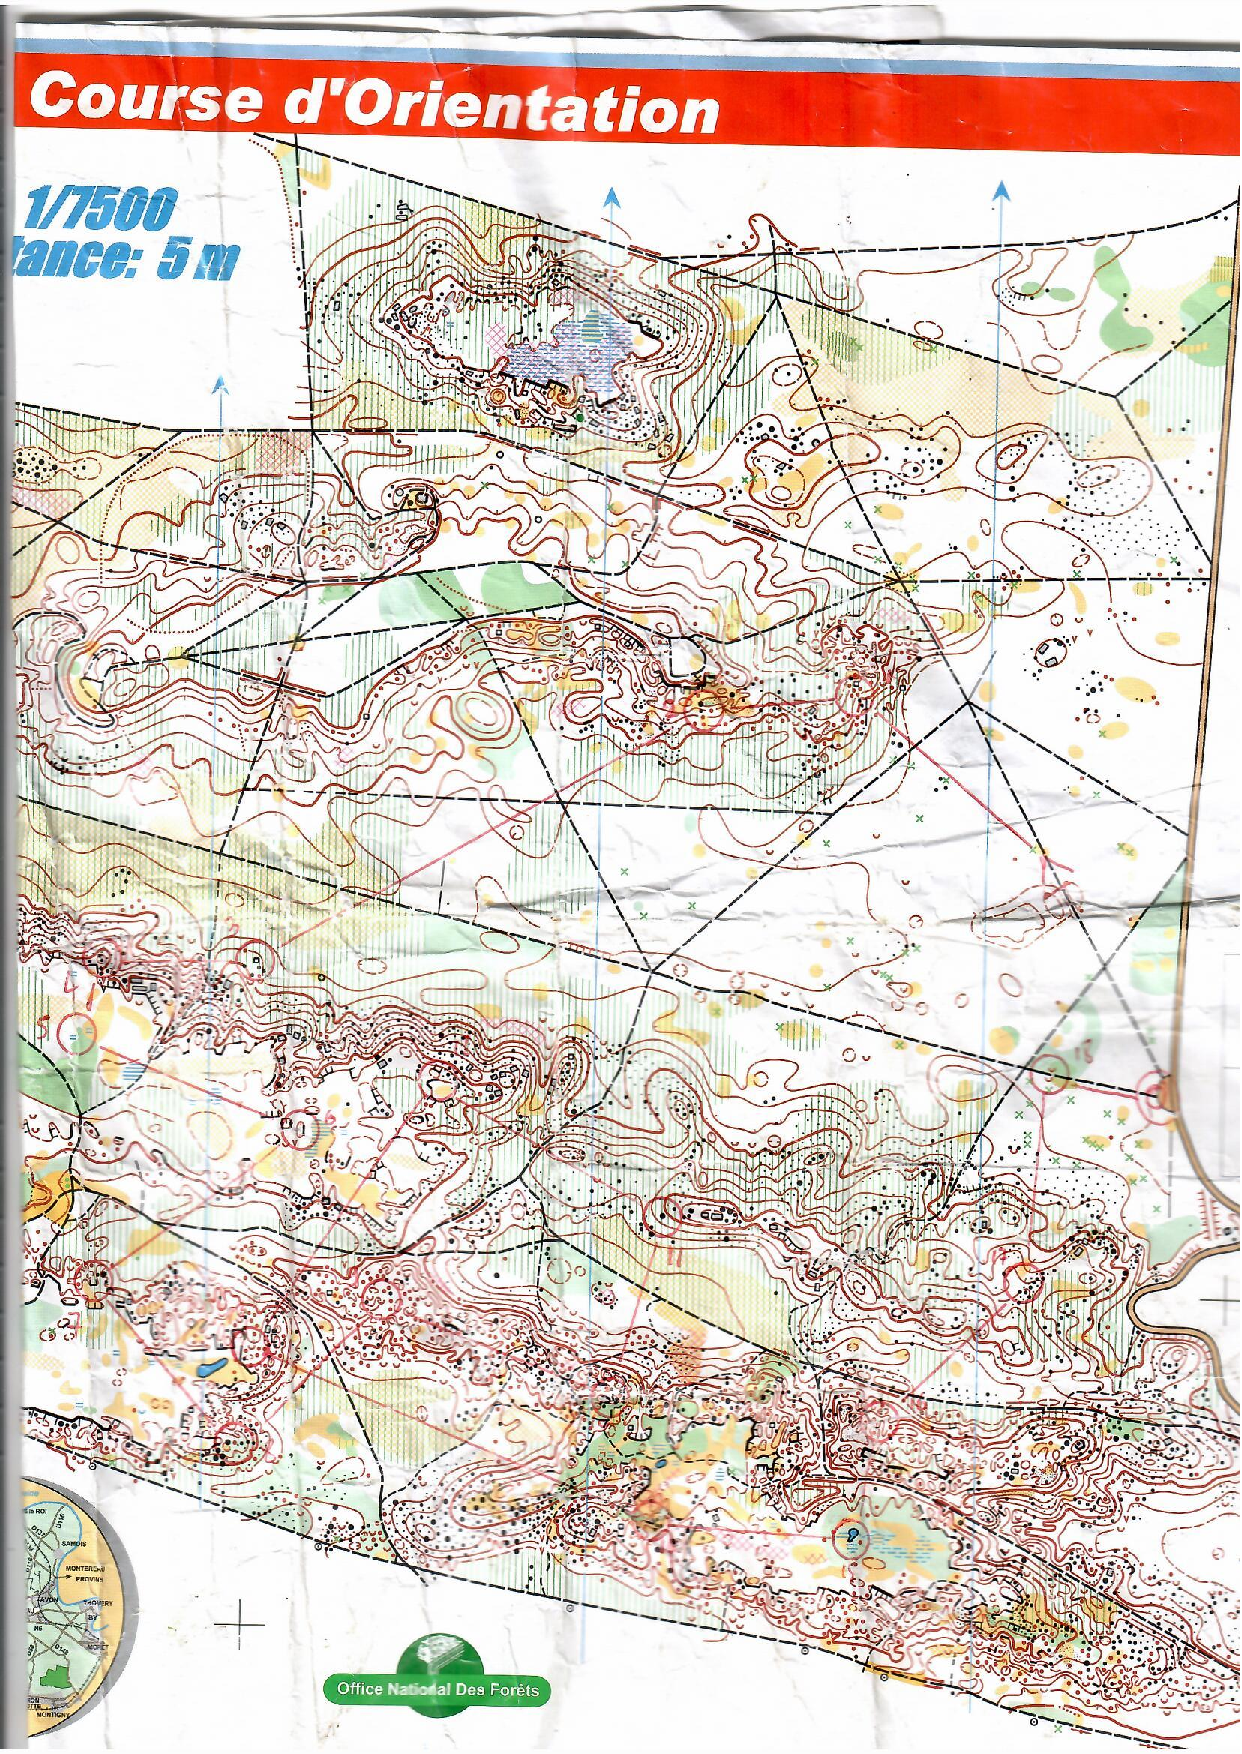
\includegraphics[width=300pt]{le-carrosse.pdf}");
%    B = TEX("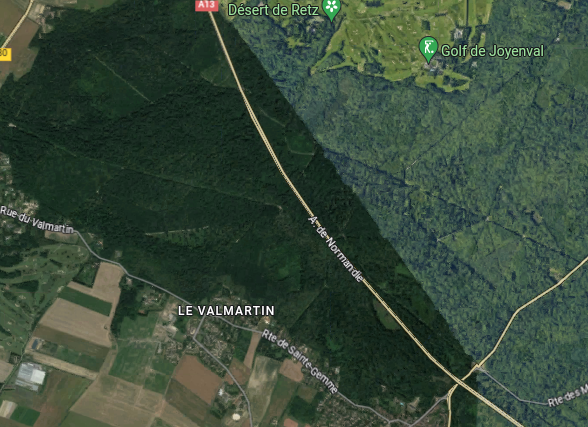
\includegraphics[width=300pt]{marly.mps}");

        xmin=3 ;
        xmax=10 ;
        ymin = 1.1 ;
        ymax = 10 ;

        %draw A ;
        numeric dx,dy,ratio ;
        dx=0;
        dy=0 ;
        ratio=1 ;
        draw A ;
%    draw B  scaled ratio shifted (dx,dy);

        fill fullcircle scaled 10 withcolor (1,0,0) ;

        path p ;
        transform t ;
        numeric scale,dx,dy;
        scale=1200;
        dx=10.0cm;
        dy=5.3cm ;
        theta=-5 ;
        t := identity scaled scale rotated theta shifted (dx,dy);
        p := get_route(t) ;

        pair pp[] ;
        pp0 = point 166 of p ;
        color pcolor ;
        pcolor = (0,1,0) ;
        draw fullcircle scaled 5 shifted pp0 withcolor pcolor ;

        pp1 = point 231 of p ;
        draw fullcircle scaled 5 shifted pp1 withcolor pcolor ;

        pp2 = point 865 of p ;
        draw fullcircle scaled 5 shifted pp2 withcolor pcolor ;

        pp3 = point 1106 of p ;
        draw fullcircle scaled 5 shifted pp3 withcolor pcolor ;


        pair qq[] ;
        color qcolor ;
        qq0 = (135,229) ;
        qcolor=(1,0,0) ;
        draw fullcircle scaled 5 shifted qq0 withcolor qcolor ;

        qq1 = (54,216) ;
        draw fullcircle scaled 5 shifted qq1 withcolor qcolor ;

        qq2 = (98,45) ;
        draw fullcircle scaled 5 shifted qq2 withcolor qcolor ;

        qq3 = (246,165) ;
        draw fullcircle scaled 5 shifted qq3 withcolor qcolor ;


        pickup pencircle scaled 1;
%        draw p withcolor pcolor ;

        transform tt[] ;
        qq0 = pp0 transformed tt0 ;
        %       qq1 = pp1 transformed tt ;
        qq2 = pp2 transformed tt0 ;
        qq3 = pp3 transformed tt0 ;

        %qq0 = pp0 transformed tt0 ;
        qq1 = pp1 transformed tt1 ;
        qq2 = pp2 transformed tt1 ;
        qq3 = pp3 transformed tt1 ;



        transform chosen_tt ;
        chosen_tt=tt0 ;

        path pp ;
        %pp = p transformed chosen_tt ;

%        draw pp withcolor (1,0,0) ;

        draw p transformed tt0 withcolor (0,0,1) ;
        draw p transformed tt1 withcolor (0,0,1) ;

%        pp = .5[p transformed tt0 ,p  transformed tt1 ] ;
%        draw pp withcolor (1,0,0) ;


        pair wpts[] ;
        get_wpts(wpts)(t) ;
        show "this is wpts" ;
        show wpts ;
        numeric i;
        i=0 ;
        forever:
                exitif unknown wpts[i] ;
                show wpts[i] ;
                pair pwpt ;
%                pwpt = wpts[i] transformed chosen_tt ;
%                draw fullcircle scaled 10 shifted pwpt withcolor (1,0,0) ;
                i:=i+1 ;
        endfor ;


        endfig;

    \end{mplibcode}

\end{document}
